\section{IMPLEMENTATION}
\begin{frame}{IMPLEMENTATION}
    \begin{figure}
        \centering
        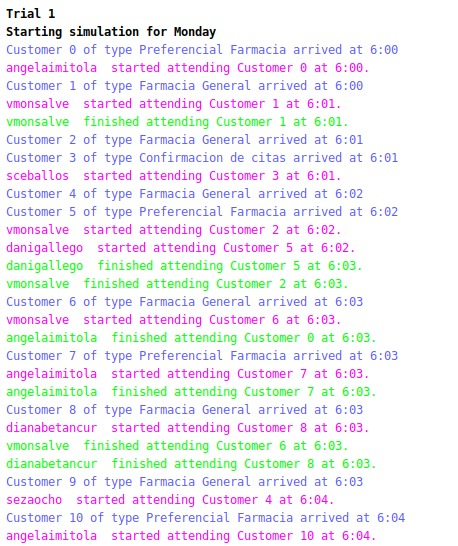
\includegraphics[scale=0.35]{images/model.jpeg}
        \caption{Model in execution.}
    \end{figure}
\end{frame}

\section{RESULTS}
\begin{frame}{RESULTS}
\begin{multicols}{2}
\begin{itemize}
    \item Nature of simulation $\rightarrow$ terminating.
    \item Output nature $\rightarrow$ transient.
    \item Biased $\rightarrow$ Not considered.
    \item Initial/final conditions $\rightarrow$ zero.
    \item Number of runs $\rightarrow$ huge.\\ 
\columnbreak
    \begin{equation*}
    n \geq\left(\frac{t_{\alpha/2;n_0-1} \times \sigma}{\delta}\right)^{2}
    \end{equation*}
\end{itemize}
\end{multicols}
\begin{figure}
    \centering
    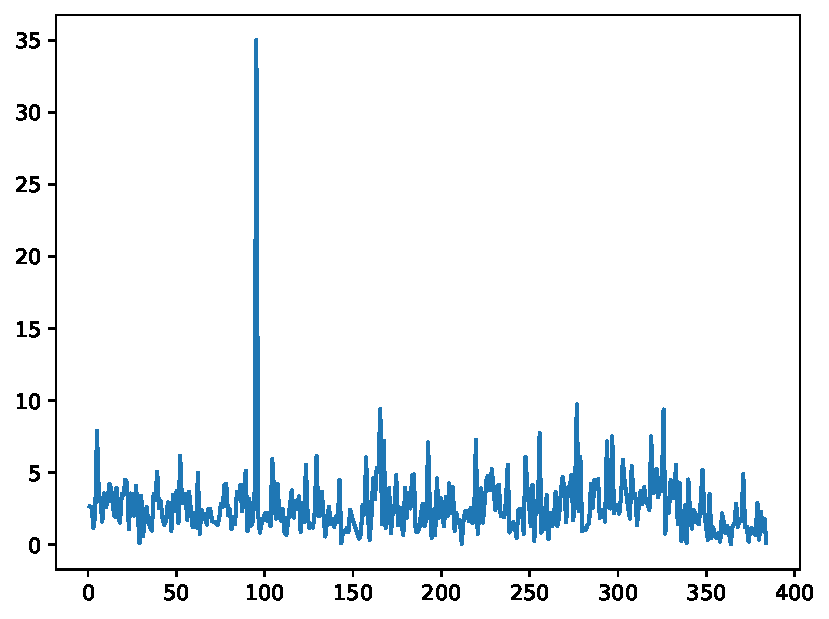
\includegraphics[scale=.4]{images/time-series.pdf}
    \caption{Time series for average waiting time in a week.}
\end{figure}
\end{frame}

\section{VERIFICATION \& VALIDATION}
\begin{frame}{VERIFICATION \& VALIDATION}
    \citep[Ch. 12]{robinson2004simulation}
    \begin{multicols}{2}
        \textbf{White-Box}
        \begin{itemize}
            \item Extreme conditions
            \item Initial conditions
            \item Distributions
            \item Priorities
        \end{itemize}
        \begin{figure}
            \centering
            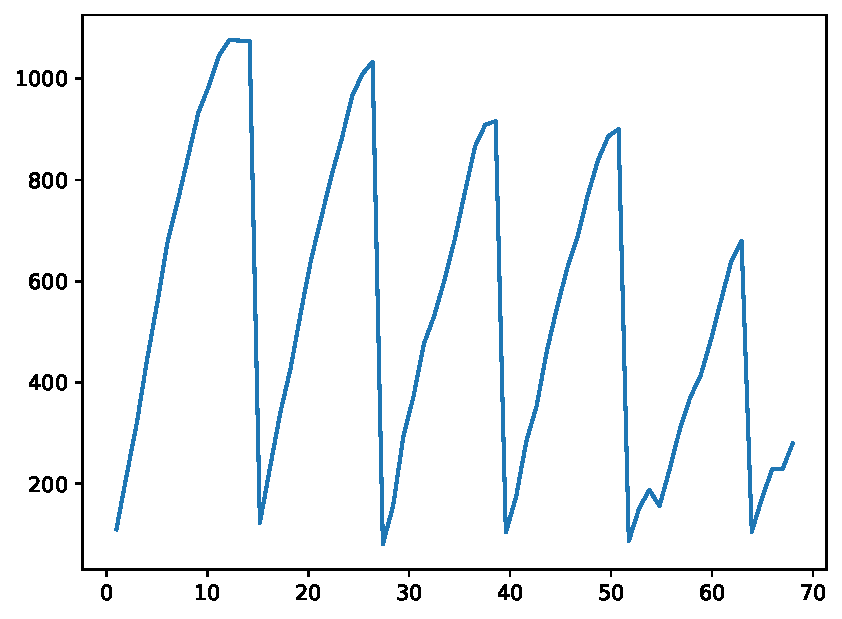
\includegraphics[scale=.35]{images/validation.pdf}
            \caption{Number of patients for each hour with one attendant.}
        \end{figure}
        \columnbreak
        \textbf{Black-Box}
        \begin{itemize}
            \item Confidence interval
        \end{itemize}
                
        \begin{equation*}
        \bar{X}_{\mathrm{S}}-\bar{X}_{R} \pm t_{\alpha / 2; 2 n-2} \sqrt{\frac{S_{S}^{2}+S_{R}^{2}}{n}}
        \end{equation*}
         \[[-55.71, -53.60]\]
    \end{multicols}
\end{frame}